\documentclass{journal}
\usepackage{graphicx}
\usepackage{siunitx}
\usepackage{caption}
\usepackage{float}

\begin{document}
\title{AP Calculus Final Project}
\author{Joshua Morin-Baxter, Alan Zhu, Nathan Wiley, and George Hong}
\date{\today}

\maketitle

\begin{abstract}
This is an analysis of data taken from the GOSH Flight Path Predictor\textsuperscript{TM}.
Four separate sets of data were analyzed:
temperature vs. density, wind velocity vs. pressure, wind angle vs. wind velocity, and wind velocity vs. altitude.
Each is discussed in more depth in subsequent parts.
\end{abstract}

\part{Wind Velocity vs. Altitude}
This data seems to have two points that are of great interest.
\begin{figure}[h]
\centering
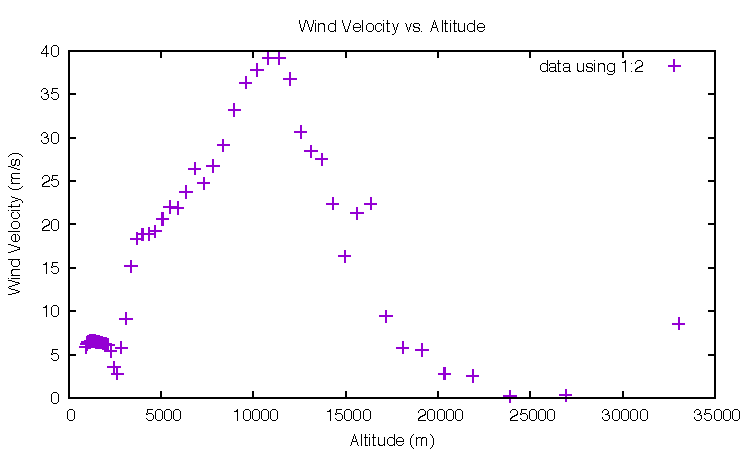
\includegraphics{josh-images/figure1.pdf}
\caption{Test}

\end{figure}


\part{Temperature Vs. Density}

\part{Wind Velocity vs. Pressure}
\begin{figure}[H]
\centering
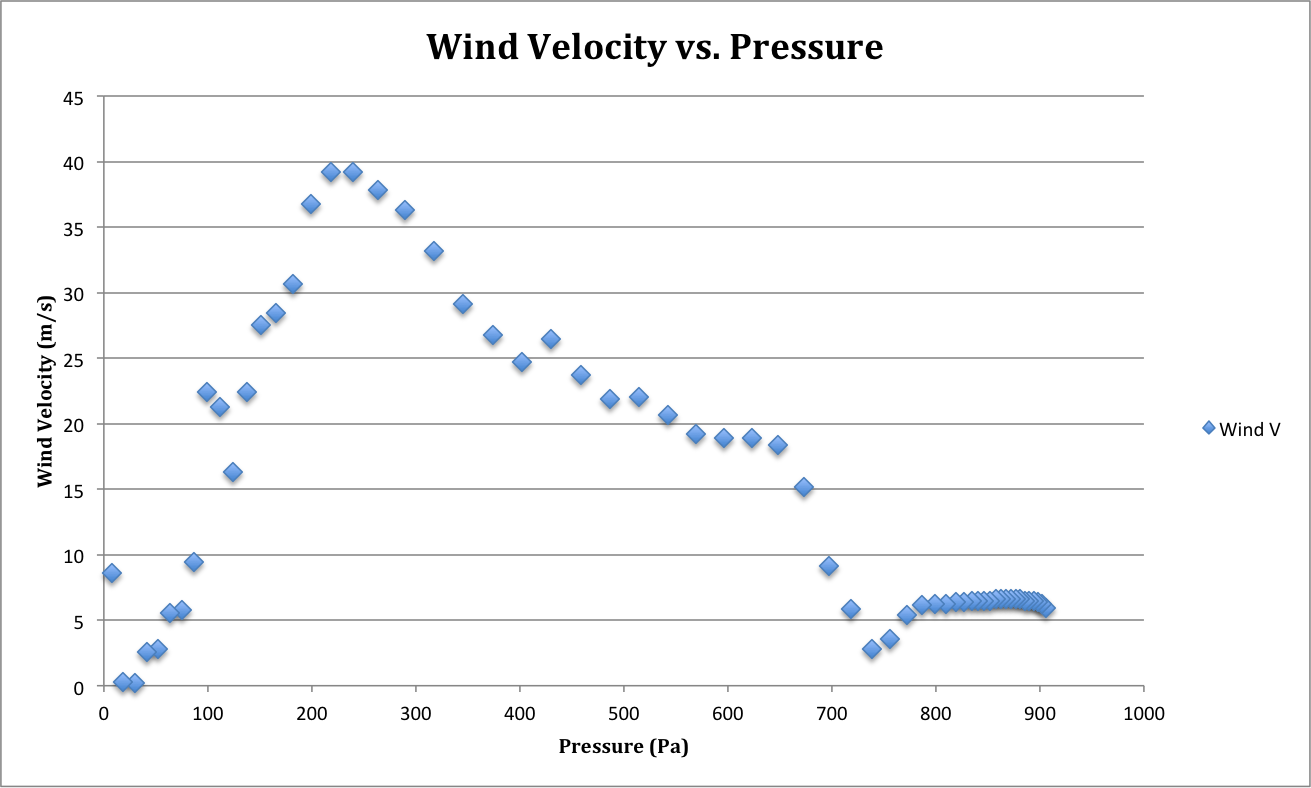
\includegraphics[width=5in]{IMG1CDATA.png}
\caption{Plot of Wind Velocity vs. Pressure}
\end{figure}

\begin{flushleft}
\textbf{Analysis:} After plotting all the points in a scatterplot, we notice our predicted concavities are well matched.  From the first derivative, we can split the data points into two distinct sections.  Pressures $\in$ [0,230) experience mostly increasing wind velocity, and Pressures $\in$ (230,725] experience primarily decreasing wind velocity.  Following a pressure of 800 Pascals, wind velocity stabilizes at $6.3\frac{m}{s} \pm 0.2\frac{m}{s}$.  We notice that wind speed is caused by shifts from high to low pressures, and the data from (230, 900) conforms to this principle: Wind speed increases as Pressure decreases.  Factors including temperature and the location of Jet Streams will result in divergence from this pattern.  Pressure is highest when altitude is lower, so the stable plateau of wind velocity at the highest pressures are expected.  Pressure collected in our data monotonically decreased with altitude.  Plots of Wind Velocity vs. Pressure or Altitude will simply be a horizontal reflection in this case.
\end{flushleft}
\part{Wind Velocity vs. Wind Angle}
\begin{figure}[H]
  \centering
  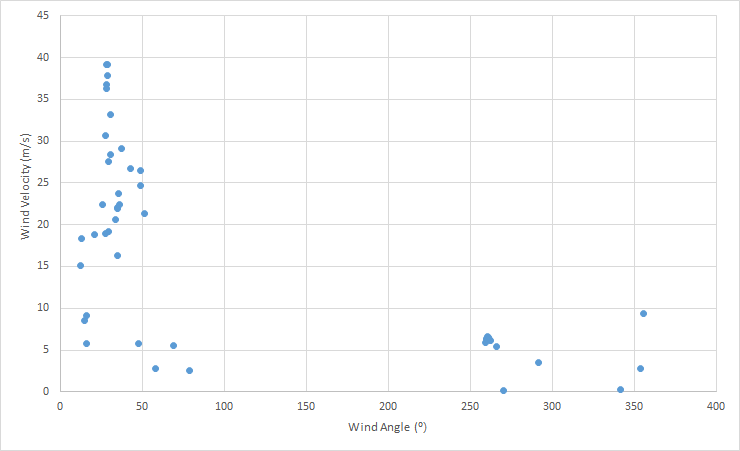
\includegraphics[width=\textwidth]{alan-data.png}
  \caption{Plot of Wind Velocity vs. Wind Angle}
\end{figure}

Although the tendencies of the data tend to wary between points, some overarching trends can be noted by analyzing the sign of the first and second derivatives (especially where they change).
The data can be analyzed on various intervals.
\begin{itemize}
  \item $angle \in (12^{\circ},16^{\circ})$: Data varies wildly.
  \item $angle \in (20^{\circ}, 28^{\circ})$ Data is almost consistently increasing, before reaching a critical point while being concave down (thus being a local maximum).
  \item $angle \in (29^{\circ}, 35^{\circ})$ Data is also almost consistently increasing.
  \item $angle \in (35^{\circ}, 37^{\circ})$ Data varies before reaching a critical point while being concave down (thus being a local maximum).
  \item $angle \in (37^{\circ}, 48^{\circ})$ Data slowly and inconsistently decreases.
  \item $angle \in (48^{\circ}, 52^{\circ})$ Decreases before reaching a critical point and point of inflection (thus being a local minimum)
  \item $angle \in (53^{\circ}, 80^{\circ})$ Data varies.
  \item $angle \in (259^{\circ}, 260.2^{\circ})$ Data is increasing and concave up before reaching a point of inflection
  \item $angle \in (260.2^{\circ}, 261^{\circ})$ Data is varying, but is critical and has a varying second derivative, meaning the data has a local maximum in this area.
  \item $angle \in (261^{\circ}, 271^{\circ})$ Data is decreasing, but second derivative goes from negative to positive, reaching a critical point where the second derivative is positive (thus being a local minimum)
  \item $angle \in (290^{\circ}, 355^{\circ})$ Data is consistently increasing, reaching a maximum at the end of the data.
\end{itemize}

The critical point on the interval $(35^{\circ}, 37^{\circ})$ and the general clustering of data around it represents the jet stream, blowing towards the NEbN (Northeast by North), while the critical point near 260 degrees seems to be the surface wind, which blows towards WbS (West by South).

The jet stream data can be fit by a normal distribution with $R = 0.536$.

\begin{figure}[H]
  \centering
  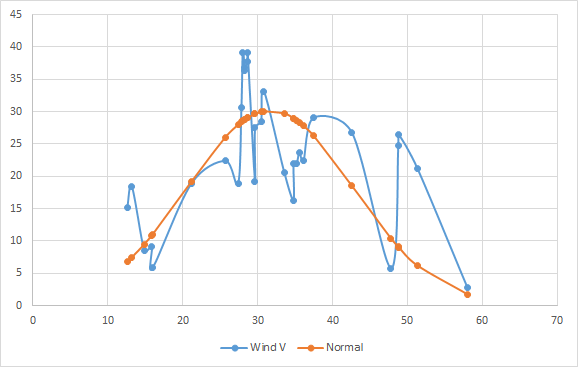
\includegraphics[width=\textwidth]{alan-data-2.png}
  \caption{Plot of Wind Velocity vs. Wind Angle on the Interval $(10^{\circ}, 60^{\circ})$ Fit by a Normal Distribution}
\end{figure}


\end{document}
